% -------------------------------------------------------------- applications part was in GAN introduction
%-------------------------------- found out that this application is not relevant
% \textbf{Applications:} GANs have been used in a wide spectrum of applications, \citet{bicycle} used \textit{Bicycle} GAN to map an input image to multiple different output images, see Fig.\ref{fig:bicycle}.
% \begin{figure}[h]
%     \centering{
%     % \includegraphics{\input{figures/bicycle.pdf}}
%     \def\svgwidth{\linewidth}
%     \input{figures/bicycle.pdf_tex}}
%     \caption{\citet{bicycle} used Bicycle GAN, input image of a scene in the evening (top left), a winter version on top right as a ground truth, in the bottom two images in a clear summer day (left) and autumn evening (right).  }
%     \label{fig:bicycle}
% \end{figure}

%--------------------------------- DCGAN training 
% \begin{algorithm*}
% \begin{algorithmic}[1]
% \FORALL{Epochs}
% \FORALL{Batches, x}
% \STATE Generator forward with a batch of random latent vectors ($z\ \in P_z; P_z=N(0,1)$) and generate a batch of fake images (Fake).
% \STATE Discriminator forward with two batches, one real (dense arrow) and one fake (dashed arrow). Output realism probability (D(x), D(G(z))).
% \STATE Calculate D loss using equation (1). Backpropagate and update D parameters using gradient decent.
% \STATE Calculate G loss for the fake batch using eq (2). Backpropagate and update G parameters using gradient decent.
% \ENDFOR
% \ENDFOR
% \end{algorithmic}
% \caption{DCGAN Training}
% \label{alg:GAN_training}
% \end{algorithm*}

\begin{figure*}
    \centering
    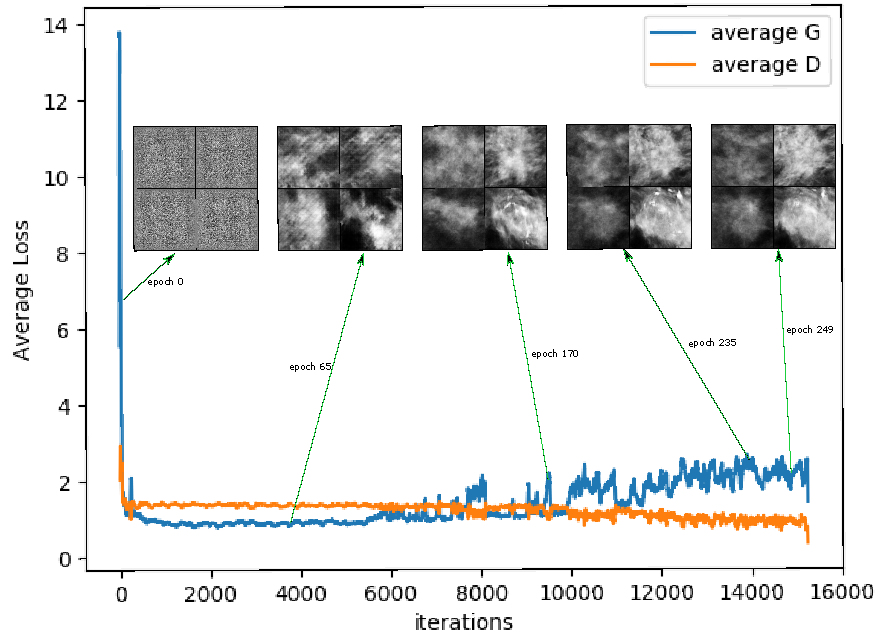
\includegraphics[scale=0.55, angle=0]{figures/GAN_progress.eps}
    \caption{GAN progress, showing 5 generated images at different points in the training process,
    these images are taken from epochs 0, 65, 170, 235, 249, where the input was fixed to four latent vectors. The horizontal axis is the training iterations, the verticla one is for binary cross entropy loss. }
    \label{fig:my_label}
\end{figure*}



\begin{figure*}
    \centering
    \includegraphics[scale=1]{figures/real_or_fake.eps}
    \caption{Two batches of real and fake images. The top one is the real batch while the bottom one is the fake one.}
    \label{fig:real_or_fake}
\end{figure*}


% In the US, 1 in every 8 women is projected to be diagnosed with breast cancer in their lifetime with a positive diagnosis rate of one every 2 minutes and death rate of one every 13 minutes. The approximate total number of breast-cancer-related deaths in the US only in 2019 is 42,260 \citep{US_stats}.